%%%%%%%%%%%%%%%%%%%%%%%%%%%%%%%%%%%%%%%%%%%%%%%%%%%%%%%%%%%%%%%%%%%%%%%%%%%%%%%
% reper w ruchu po okręgu
%%%%%%%%%%%%%%%%%%%%%%%%%%%%%%%%%%%%%%%%%%%%%%%%%%%%%%%%%%%%%%%%%%%%%%%%%%%%%%%
\subsection{Ruch po okręgu wokół czarnej dziury}
W układzie obserwatora inercjalnego $\mathcal{I}$ z~sferycznym układem
współrzędnych $(t,r,\phi,\theta)$ rozważamy linię świata 
obserwatora $\mathcal{Z}$ w ruchu jednostajnym po okręgu wokół czarnej dziury.
Będziemy używać metryki Schwarzschilda, która odpowiada 
czasoprzestrzeni w pobliżu nierotującej sferycznie symetrycznej masie 
nieobdarzonej ładunkiem~\cite{hartle2016}. 
Element liniowy oraz macierz tensora metrycznego mają postać
\begin{align} \label{CDlin}
\d s^2 = 
 \left(1-\frac{2 M}{r}\right) \d t^2 
 -\left(1-\frac{2 M}{r}\right)^{-1} \d r^2 
 -r^2 \sin ^2\theta\d \phi^2 
 -r^2 \d \theta^2.
\end{align}
\begin{align}\label{CDmetric}
(g_{\mu\nu}) = \left(
\begin{array}{cccc}
 1-\frac{2 M}{r} & 0 & 0 & 0 \\
 0 & -\left(1-\frac{2 M}{r}\right)^{-1} & 0 & 0 \\
 0 & 0 & -r^2 \sin ^2\theta  & 0 \\
 0 & 0 & 0 & -r^2 \\
\end{array}
\right).
\end{align}
Dla metryki~\eqref{CDmetric} symbole Christoffela $\Gamma^k _{ij}$ 
przedstawiam poniżej w tablicach odpowiednio dla $k=0,1,2,3$
$$
\left(
\begin{array}{cccc}
 0 & \frac{M}{r^2}\left( 1 - \frac{2M}{r}  \right)^{-1}& 0 & 0 \\
 \frac{M}{r^2}\left( 1 - \frac{2M}{r}  \right)^{-1} & 0 & 0 & 0 \\
 0 & 0 & 0 & 0 \\
 0 & 0 & 0 & 0 \\
\end{array}
\right),\left(
\begin{array}{cccc}
 \frac{M}{r^2}\left( 1 - \frac{2M}{r}  \right) & 0 & 0 & 0 \\
 0 &-\frac{M}{r^2}\left( 1 - \frac{2M}{r}  \right)^{-1} & 0 & 0 \\
 0 & 0 & -\left(1-\frac{2M}{r}\right)r \sin ^2\theta  & 0 \\
 0 & 0 & 0 & -r \left(1-\frac{2M}{r}\right) \\
\end{array}
\right),
$$
$$
\left(
\begin{array}{cccc}
 0 & 0 & 0 & 0 \\
 0 & 0 & \frac{1}{r} & 0 \\
 0 & \frac{1}{r} & 0 & \frac{\cos \theta}{\sin\theta}  \\
 0 & 0 &\frac{ \cos \theta }{\sin \theta }  & 0 \\
\end{array}
\right),\left(
\begin{array}{cccc}
 0 & 0 & 0 & 0 \\
 0 & 0 & 0 & \frac{1}{r} \\
 0 & 0 & -\cos \theta\sin \theta  & 0 \\
 0 & \frac{1}{r} & 0 & 0 \\
\end{array}
\right)
$$
Jak poprzednio rozważamy ruch po okręgu o promieniu $R$ i częstości $\omega$.
W rozważanym układzie współrzędnych linię świata można zapisać następująco
%W tym układzie punkt
%poruszający się po okręgu o promieniu $R$ i częstości $\omega$ w układzie
%obserwatora inercjalnego $\mathcal{I}$ porusza się po 
%trajektorii~$y=y(s)$. Współrzędne trajektorii w układzie
%kartezjańskim obserwatora~$\mathcal{I}$ mają postać
%Zapis współrzędnych bez oznaczenia będziemy 
%rozumieć jako współrzędne w bazie kanonicznej.
\begin{equation}\label{y_CD}
(y^\mu) = \left( t,\ R,\ \omega t,\ \frac{\pi}{2}\right).
\end{equation}
Wtedy wektor prędkości ma postać
\begin{equation}\nonumber
(u^\mu) = \left( \frac{\d y^\mu}{\d s} \right) 
= (\gamma,\ 0,\ \omega\gamma,\ 0),
\end{equation}
gdzie $\gamma = \d t/\d s$. Z danego elementu liniowego~\eqref{CDlin}, 
po uwzględnieniu~\eqref{y_CD}, możemy odczytać 
\begin{align}\nonumber
\gamma = \frac{\d t}{\d s} = 
 \left(1 - \frac{2 M}{R} - R^2\omega^2 \right)^{-1/2}.
\end{align}
Wyznaczamy przyspieszenie oraz przyspieszenie właściwe
\begin{align}\nonumber
(A^\mu) = \left(0,\ -\gamma^2 \left( R\omega^2 - \frac{M}{R^2} \right) 
\left(1-\frac{2M}{R}\right),\ 0,\ 0 \right)
\end{align}
\begin{align}\nonumber
\alpha = \sqrt{-A\cdot A} = \gamma^2 
\left| R\omega^2 - \frac{M}{R^2} \right|
\left( 1-\frac{2M}{R} \right)^{1/2}
\end{align}

Ponownie skorzystamy z bazy wyznaczonej wcześniej dla przypadku
czasoprzestrzeni Minkowskiego i uogólnimy ją w ten sposób, 
aby była unormowana i spełniała prawo transportu~\eqref{FW}.
Takie postępowanie daje nam łatwy sposób sprawdzania poprawności
obliczeń, gdyż dla $M=0$ wyniki powinny przechodzić w przypadek 
bez grawitacji, czyli czasoprzestrzeń Minkowskiego.
W pierwszym kroku musimy przetransformować wektory bazy~\eqref{Esimple}
do współrzędnych sferycznych.  Na potrzeby tej transformacji
współrzędne kartezjańskie oznaczymy przez $x^i$, natomiast współrzędne 
sferyczne przez $\tilde{x}^i$. Współrzędne wektorów transformują 
się kontrawariantnie~\cite{inga1980} co można zapisać jako
\begin{align}\nonumber
\tilde{v}^i = \frac{\partial \tilde{v}^i}{\partial v^j} v^j.
\end{align}
Współczynniki tej transformacji obliczamy w punkcie należącym do 
rozważanej tu linii świata. Baza~\eqref{Esimple} we współrzędnych sferycznych
ma zatem postać 
\begin{align}\nonumber
\widetilde{E}=
\begin{pmatrix}
e_0\\
e_1\\
e_2\\
e_3
\end{pmatrix}
=
\begin{pmatrix}
\gamma & 0 & \gamma \omega & 0 \\
R\omega\gamma \sin \psi & \cos\psi & \frac{\gamma}{R} \sin\psi & 0\\
R\omega\gamma \cos \psi & -\sin\psi & \frac{\gamma}{R} \cos\psi & 0\\
0 & 0 & 0 & -\frac{1}{R} \\
\end{pmatrix}.
\end{align}
Powyższa baza, rozważana w czasoprzestrzeni z metryką
Schwarzschilda, nie jest ortonormalna. Można jednak stosunkowo łatwo
uogólnić ją w ten sposób aby ortonormalna była
\begin{align}\nonumber
\widetilde{E}=
\begin{pmatrix}
e_0\\
e_1\\
e_2\\
e_3
\end{pmatrix}
=
\begin{pmatrix}
\gamma & 0 & \gamma \omega & 0 \\
R\omega\gamma \sin \psi \left(1-\frac{2 M}{R} \right)^{-1/2} 
& \cos\psi\left(1-\frac{2 M}{R} \right)^{1/2} 
& \frac{\gamma}{R} \sin\psi\left(1-\frac{2 M}{R} \right)^{1/2} & 0\\
R\omega\gamma \cos \psi\left(1-\frac{2 M}{R} \right)^{-1/2} 
& -\sin\psi \left(1-\frac{2 M}{R} \right)^{1/2}
& \frac{\gamma}{R} \cos\psi \left(1-\frac{2 M}{R} \right)^{1/2}& 0\\
0 & 0 & 0 & -\frac{1}{R} \\
\end{pmatrix}.
\end{align}
Odpowiedni kąt obrotu~$\psi$ znajdujemy za pomocą prawa transportu~\eqref{FW}.
Dają one równania różniczkowe (jak poprzednio zakładamy $\psi(0)=0$), 
które mają wspólne rozwiązanie dane przez~\eqref{PsiCD}.
\begin{align}\label{PsiCD}
\psi = - \omega \gamma^2 s \left( 1-\frac{3M}{R} \right).
\end{align}
Mając odpowiedni reper ruchomy znajdujemy równanie na 
fazę zegara~\eqref{PhiCD}
\begin{align}\nonumber
\chi &= - \psi =\omega \gamma^2 s \left( 1-\frac{3M}{R} \right)
 , \quad 
\alpha =  \gamma^2 
\left| R\omega^2 - \frac{M}{R^2} \right|
\left( 1-\frac{2M}{R} \right)^{1/2}
\\
\dot{\varphi} &= \pm \frac{2}{\ell} + \label{PsiCD}
\gamma^2 
\left| R\omega^2 - \frac{M}{R^2} \right|
\left( 1-\frac{2M}{R} \right)^{1/2}
\sin \left(\varphi - 
\omega \gamma^2 s \left( 1-\frac{3M}{R} \right)
 \right)
\end{align}


Zauważmy, że uzyskane równanie różni się od rozwiązania 
otrzymanego w ruchu po okręgu w 
płaskiej metryce Minkowskiego czynnikami
$\left( 1-2M/R \right)^{1/2}$,
$ \left( 1-3M/R \right)$, $-M/R^2$ oraz czynnikiem w $\gamma$. 
Ze wzrostem promienia najszybciej można zaniedbać czynnik 
proporcjonalny do $1/R^2$. 
Porównanie wagi każdego z czynników
w zależności od $R$ 
przedstawiamy na wykresie~\ref{CD1plot}.
Dla uproszczenia porównania oraz lepszego oddania kreślimy 
wykres $1-M/R^2$ zamiast $M/R^2$. Pomijamy w analizie 
czynnik $\gamma$,
 gdyż zbiega on do odpowiednika w metryce Minkowskiego
podobnie jak $\left( 1-2M/R \right)^{1/2}$.
Dla odpowiednio dużych $R$ wpływ masy $M$ na działanie zegara jest niewielki, 
przy czym silniej wpływa na $\chi$ niż na $\alpha$.  
\begin{figure}
\centering
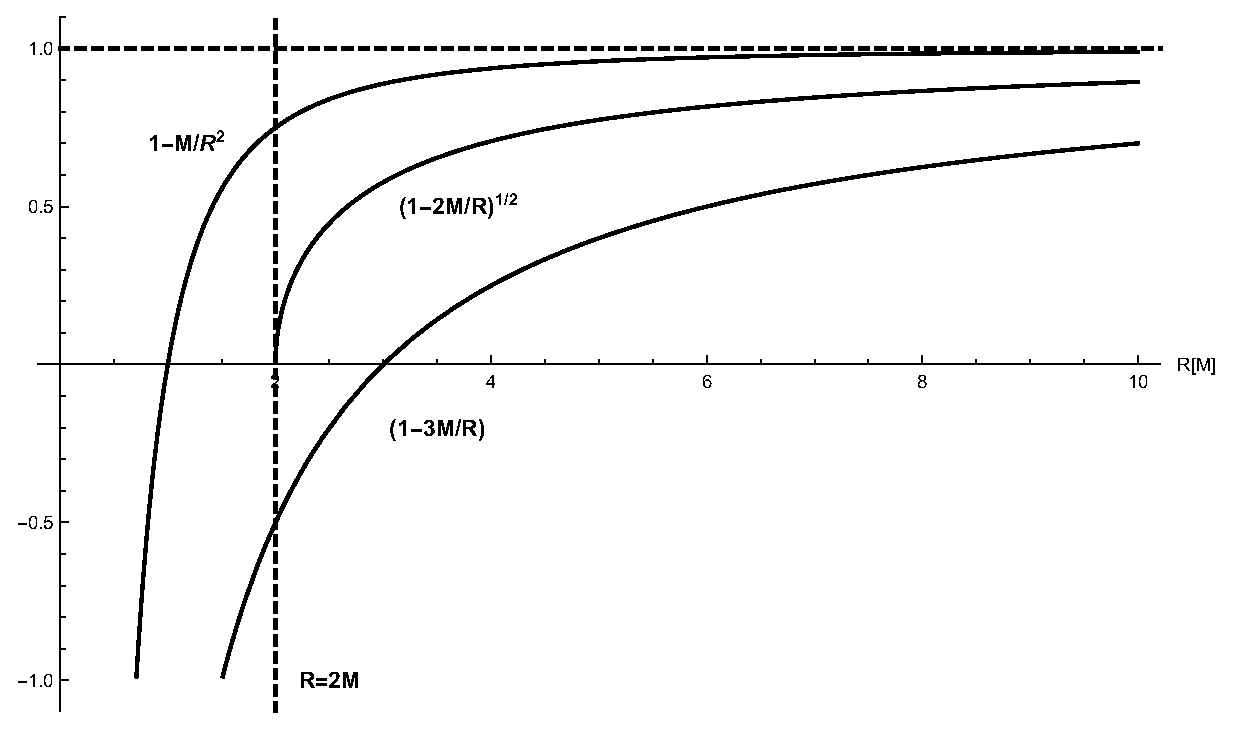
\includegraphics[scale=0.6]{CD1.eps}
\caption{Wykres czynników wpływających na działanie zegara 
pochodzących od $M$ w zależności od $R$.}{\label{CD1plot}}
\end{figure}

Jeśli zamiast ruchu po okręgu rozważymy zegar spoczywający w 
polu grawitacyjnym odpowiednie rachunki przebiegają podobnie i 
wystarczy w powyższych rozważaniach położyć $\omega=0$.
Otrzymujemy wtedy 
\begin{align*}
\gamma &= \left( 1 - \frac{M}{R^2} \right)^{-1/2},\\
\alpha &= \frac{M}{R^2} \left( 1 - \frac{M}{R^2} \right)^{1/2},\\
\chi &= 0,\\
\dot{\varphi} &= \pm \frac{2}{\ell} +
\gamma^2  \frac{M}{R^2} 
\left( 1-\frac{2M}{R} \right)^{1/2}
\sin \left(\varphi  \right).
\end{align*}
W przypadku zegara spoczywającego w polu grawitacyjnym 
struktura równania na fazę przypomina równanie uzyskane 
dla ruchu hiperbolicznego, co sugeruje, że działanie 
zegara w tych przypadkach może być podobne.  
